\chapter{CTMQC applied to molecular systems}
\label{chap:molecular_systems}
In order to apply CTMQC to large molecular systems (hundreds of molecules) a different way to construct the Hamiltonian is needed. In this work I have implemented the CTMQC equations within the fragment-orbital based framework. This relies on the equations being expressed in a pseudo-diabatic basis and the Hamiltonian being constructed in 2 parts: the diagonal elements (site energies) and the off-diagonals (electronic couplings). The basis is termed `pseudo-diabatic' due to the fact that non-adiabatic coupling vectors are small but non vanishing, this results in a basis where the excess charge carrier is strongly but not strictly localised on a single molecule. Within the Hamiltonian, the site energies (diagonal elements) are calculated via classical force-fields and the electronic couplings (off-diagonals) are calculated via the analytic overlap method \cite{gajdos_ultrafast_2014, spencer_fob-sh:_2016} (AOM). In this method the coupling elements are assumed to be proportional to the overlap between the highest singly occupied molecular orbitals (SOMO) on the donor and acceptor molecules (see equation \eqref{eq:AOM_proportional}). This approximation is often used in the literature, e.g. in the fragment orbital density functional theory \cite{KirkpatrickJ2008,C2CP41348E,TroisiA2002} (FODFT) method and has been shown to be valid for many $\pi$-conjugated molecules \cite{KubasA2014, gajdos_ultrafast_2014}.
\begin{equation}
  H_{ab} = C \langle \varphi_{a} | \varphi_{b} \rangle = C S_{ab}
  \label{eq:AOM_proportional}
\end{equation}
Where $\varphi_{a(b)}$ represents a singly occupied molecular orbital on the donor (acceptor) and C is the scaling constant and comes from DFT parameterisation. The singly occupied molecular orbitals are calculated as a linear combination of Slater-type orbitals (STO) as in equation  \eqref{eq:SOMO_def}. In this equation we loop over each atom in the molecule and sum the size of the contribution, $c_{p\pi, i}$, multiplied by the STO, $p_{\pi, j}$. In this case the STO is represented by a p-orbital. The size of the p-orbital on each atom, $c_{p\pi, i}$, is parameterised before the simulation with DFT.
\begin{equation}
  | \varphi_{mol} \rangle = \sum_{i \in mol}^{N_{\text{atoms}}} c_{p\pi, i} | p_{\pi, i} \rangle
  \label{eq:SOMO_def}
\end{equation}
Importantly, the AOM method offers a very fast way to calculate the off-diagonal elements of the hamiltonian via a finite-difference method with an accuracy comparable to that of DFT methods \cite{AOM_vs_HigherOrder}. This has been implemented within an open-source software package named CP2K and is used by a fragment-orbital based surface hopping technique to study large systems of hundreds of molecules. In the next chapter, the surface hopping technique will be discussed in further detail and applied to a system of pentacene molecules in order to investigate charge carrier (hole) transfer within amorphous systems.


\section{Basis Transformation}
In order to use the FOB method, as stated above, the CTMQC equations in the adiabatic basis must be transformed to the diabatic basis. In the following derivation $C_{l}$ will represent the adiabatic expansion coefficient corresponding to state l and $u_{l}$ will represent the orthogonal diabatic expansion coefficients.
\\\\
The CTMQC equations in the adiabatic basis are given below in equation \eqref{eq:adForce} of the forces and \eqref{eq:adCoeff} coefficients:
\begin{align}
  \begin{split}
	  \mathbf{F}_{\nu}^{(I)} = &- \sum_{k} |C_{k}^{(I)}|^2 \nabla_{\nu}E_{k}^{(I)} - \sum_{k, l} C_{l}^{* (I)} C_{k}^{(I)} \left(E_{k}^{(I)} - E_{l}^{(I)} \right) \mathbf{d}_{\nu, lk}^{ad, (I)} \\
	  &- \sum_{l,k} |C_{l}^{(I)}|^2 \left( \sum_{\nu'}^{N_{n}} \frac{2}{\hbar M_{\nu'}} \mathcal{Q}_{\nu', lk}^{(I)} \cdot \mathbf{f}_{l, \nu'}^{(I)} \right)\left[ \mathbf{f}_{k, \nu}^{(I)} - \mathbf{f}_{l, \nu}^{(I)} \right] |C_{k}^{(I)}|^2 
  \end{split}
  \label{eq:adForce}
\end{align}

\begin{align}
  \begin{split}
	\dot{C}_{l}^{(I)} = &-\frac{i}{\hbar} E_{l}^{(I)} C_{l}^{(I)} - \sum_{k} C_{k}^{(I)} \sum_{\nu=1}^{N_{n}} \frac{\mathbf{P}_{\nu}^{(I)}}{M_{\nu}} \cdot \mathbf{d}_{\nu, lk}^{ad, (I)} \\
	&- \sum_{\nu=1}^{N_{n}} \sum_{k} \frac{\mathcal{Q}_{\nu, lk}^{(I)}}{\hbar M_{\nu'}} \cdot \left[\mathbf{f}_{k, \nu}^{(I)} - \mathbf{f}_{l, \nu}^{(I)} \right] |C_{k}^{(I)}|^2 C_{l}^{(I)}
  \end{split}
  \label{eq:adCoeff}
\end{align}

\noindent Where:
\begin{itemize}
  \item $E_{l}^{(I)}$ is the adiabatic energy for state l and trajectory I
  \item $C_{k}^{(I)}$ is the adiabatic expansion coefficient for state k and trajectory I
  \item $\mathbf{P}_{\nu}^{(I)}$ is the classical momentum of atom $\nu$ on trajectory $I$
  \item $\mathbf{d}_{\nu, lk}^{ad, (I)}$ is the nonadiabatic coupling vector (given in the adiabatic basis)
  \item $M_{\nu}$ is the mass of nuclei $\nu$
  \item $\mathcal{Q}_{\nu, lk}^{(I)}$ is the quantum momentum vector for atom $\nu$ corresponding to the $lk$ pair of states in trajectory $I$
  \item $\mathbf{f}_{l, \nu}^{(I)}$ is the adiabatic momentum on state l, atom $\nu$ and trajectory $I$
\end{itemize}

\subsection{Coefficients}
To transform the equation for the propagation of the coefficients it is far neater to use the notation of linear algebra as in equation \eqref{eq:LA_Coeff} below:
\begin{equation}
	\dot{\mathbf{C}}^{(I)} = \mathbb{X}_{\nu}^{(I)} \mathbf{C}^{(I)} = \left(\mathbb{X}_{eh, \nu}^{(I)} + \mathbb{X}_{qm, \nu}^{(I)}\right) \mathbf{C}^{(I)}
	\label{eq:LA_Coeff}
\end{equation}
Where the $\mathbb{X}$ matrices are defined as in equations \eqref{eq:Xeh_def} and \eqref{eq:Xqm_def} below.
\begin{equation}
  \mathbb{X}_{lk, \nu}^{eh (I)} = -\frac{i}{\hbar} E_{l}^{(I)} - \sum_{\nu}^{N_{n}}\frac{\mathbf{P}_{\nu}^{(I)}}{M_{\nu}} \cdot d_{lk, \nu}^{ad, (I)}
  \label{eq:Xeh_def}
\end{equation}

\begin{equation}
  \mathbb{X}_{ll, \nu}^{qm (I)} = -\sum_{\nu=1}^{N_{n}} \sum_{k} \frac{\mathcal{Q}_{\nu, lk}^{(I)}}{\hbar M_{\nu'}} \cdot \left[ \mathbf{f}_{k, \nu}^{(I)} - \mathbf{f}_{l, \nu}^{(I)} \right]  |C_{k}^{(I)}|^2
  \label{eq:Xqm_def}
\end{equation}

\noindent Using the identities:
\begin{align}
  \mathbb{U}^{-1} &= \mathbb{U}^{\dagger} \\
  \mathbf{C}^{(I)} &= \mathbb{U}^{\dagger (I)} \mathbf{u}^{(I)} \\
  \dot{\mathbf{C}}^{(I)} &= \dot{\mathbb{U}^{\dagger (I)}} \mathbf{u}^{(I)} + \mathbb{U}^{\dagger (I)}\dot{\mathbf{u}}^{(I)}
\end{align}
Where $\mathbb{U}^{(I)} = \langle \phi_{l}^{(I)} | \psi_{n}^{(I)} \rangle$ is the unitary transformation matrix transforming from the diabatic to adiabatic basis. The $\mathbf{u}^{(I)}$ terms are the diabatic expansion coefficients on trajectory I.
\\\\
\noindent After some algebra we arrive at:
\begin{equation}
  \dot{\mathbf{u}}^{(I)} = \underbrace{\left(\mathbb{U}^{(I)} \mathbb{X}_{eh} \mathbb{U}^{\dagger (I)} + \mathbb{U}^{(I)}\mathbb{U}^{\dagger (I)}\right) \mathbf{u}^{(I)}}_{\text{Ehrenfest}} + \underbrace{\left(\mathbb{U}^{(I)} \mathbb{X}_{qm} \mathbb{U}^{\dagger (I)} \right) \mathbf{u}^{(I)}}_{\text{Quantum Momentum}}
  \label{eq:diabMatEq}
\end{equation}
In equation \eqref{eq:diabMatEq} I've separated the contribution from Ehrenfest and the contribution from the new quantum momentum terms. The Ehrenfest part can be shown to reduce to a simpler form (see Spencer, 2016 \cite{spencer_fob-sh:_2016} and Carof, 17 \cite{carof_detailed_2017} for more details). The quantum momentum term must be coded up as shown -with the transformation matrices. This gives the final equation for the propagation of the diabatic expansion coefficients, shown in equation \eqref{eq:DiabPropagation}.
\begin{equation}
  \dot{\mathbf{u}}^{(I)} = \left(-\frac{i}{\hbar} \mathbb{H}^{(I)} - \mathbb{D}^{(I)}_{diab} \right) \mathbf{u}^{(I)} + \left(\mathbb{U}^{(I)} \mathbb{X}_{qm} \mathbb{U}^{(I)})^{-1} \right) \mathbf{u}^{(I)}
  \label{eq:DiabPropagation}
\end{equation}
Where $\mathbb{H}^{(I)}$ is the diabatic Hamiltonian constructed via the AOM method, $\mathbb{D}_{diab}^{(I)}$ are the diabatic nonadiabatic coupling elements ($d_{diab, lk}^{(I)} = \langle \phi_{l} | \dot{\phi}_{k} \rangle$).

\subsection{Forces}
A full derivation of the transformation of basis for the equation propagating forces is given in appendix \ref{ap:BasisTrans}. The result is given in equation \eqref{eq:diabForces} below:
\begin{align}
  \begin{split}
	  \mathbf{F}_{eh, \nu}^{(I)} &= \sum_{i,j} \mathbf{u}_{i}^{*(I)} \mathbf{u}_{j}^{(I)} \left( \nabla_{\nu} H_{ij}^{(I)} + \sum_{l} \mathbf{d}_{lk, \nu}^{(I)} H_{lj}^{(I)} - \sum_{l} \mathbf{d}_{lj, \nu}^{(I)} H_{il} \right) \\
	  &- \sum_{l,k} |C_{l}^{(I)}|^2 \left( \sum_{\nu'}^{N_{n}} \frac{2}{\hbar M_{\nu'}} \mathcal{Q}_{\nu', lk}^{(I)} \cdot                   \mathbf{f}_{l, \nu'}^{(I)} \right)\left[ \mathbf{f}_{k, \nu}^{(I)} -          \mathbf{f}_{l, \nu}^{(I)} \right] |C_{k}^{(I)}|^2
	\end{split}
  \label{eq:diabForces}
\end{align}
Where the definitions of the terms within equation \eqref{eq:diabForces} have been explained previously.

\noindent There are a couple of things to note with this equation. Firstly, (as in the coefficients equation) the quantum momentum part has not been transformed. This is because the forces are basis independent and don't need to be transformed. Secondly, the quantities required for the calculation of this part of the equation are already calculated in order to propagate the coefficients so only a small amount of extra effort is required to calculate the quantum momentum force term. The Ehrenfest part of the equation has been transformed. This is because the nonadiabatic coupling vectors within the adiabatic basis are never required so are never calculated. The Ehrenfest force term requires these nonadiabatic coupling vectors so would add an extra computational overhead. Further, the commutator term in the diabatic basis has been observed to provide a negligible contribution to the overall force in previous simulations (not shown in this work). This term requires significant computational effort and can be neglected. This makes the calculation of the Ehrenfest forces in the diabatic basis far cheaper than in the adiabatic basis.

\section{Testing the diabatic propagator}
The diabatic propagation can be tested against the already tested adiabatic propagator using the Tully model Hamiltonian. The code should give the same results, given the same inputs. To check this, in figure \ref{fig:diab_prop_vs_adiab}, the simulations carried out in figure \ref{fig:LitCompCTMQCTullyHigh} were repeated though this time the diabatic propagator was used.
\begin{figure}[ht]
  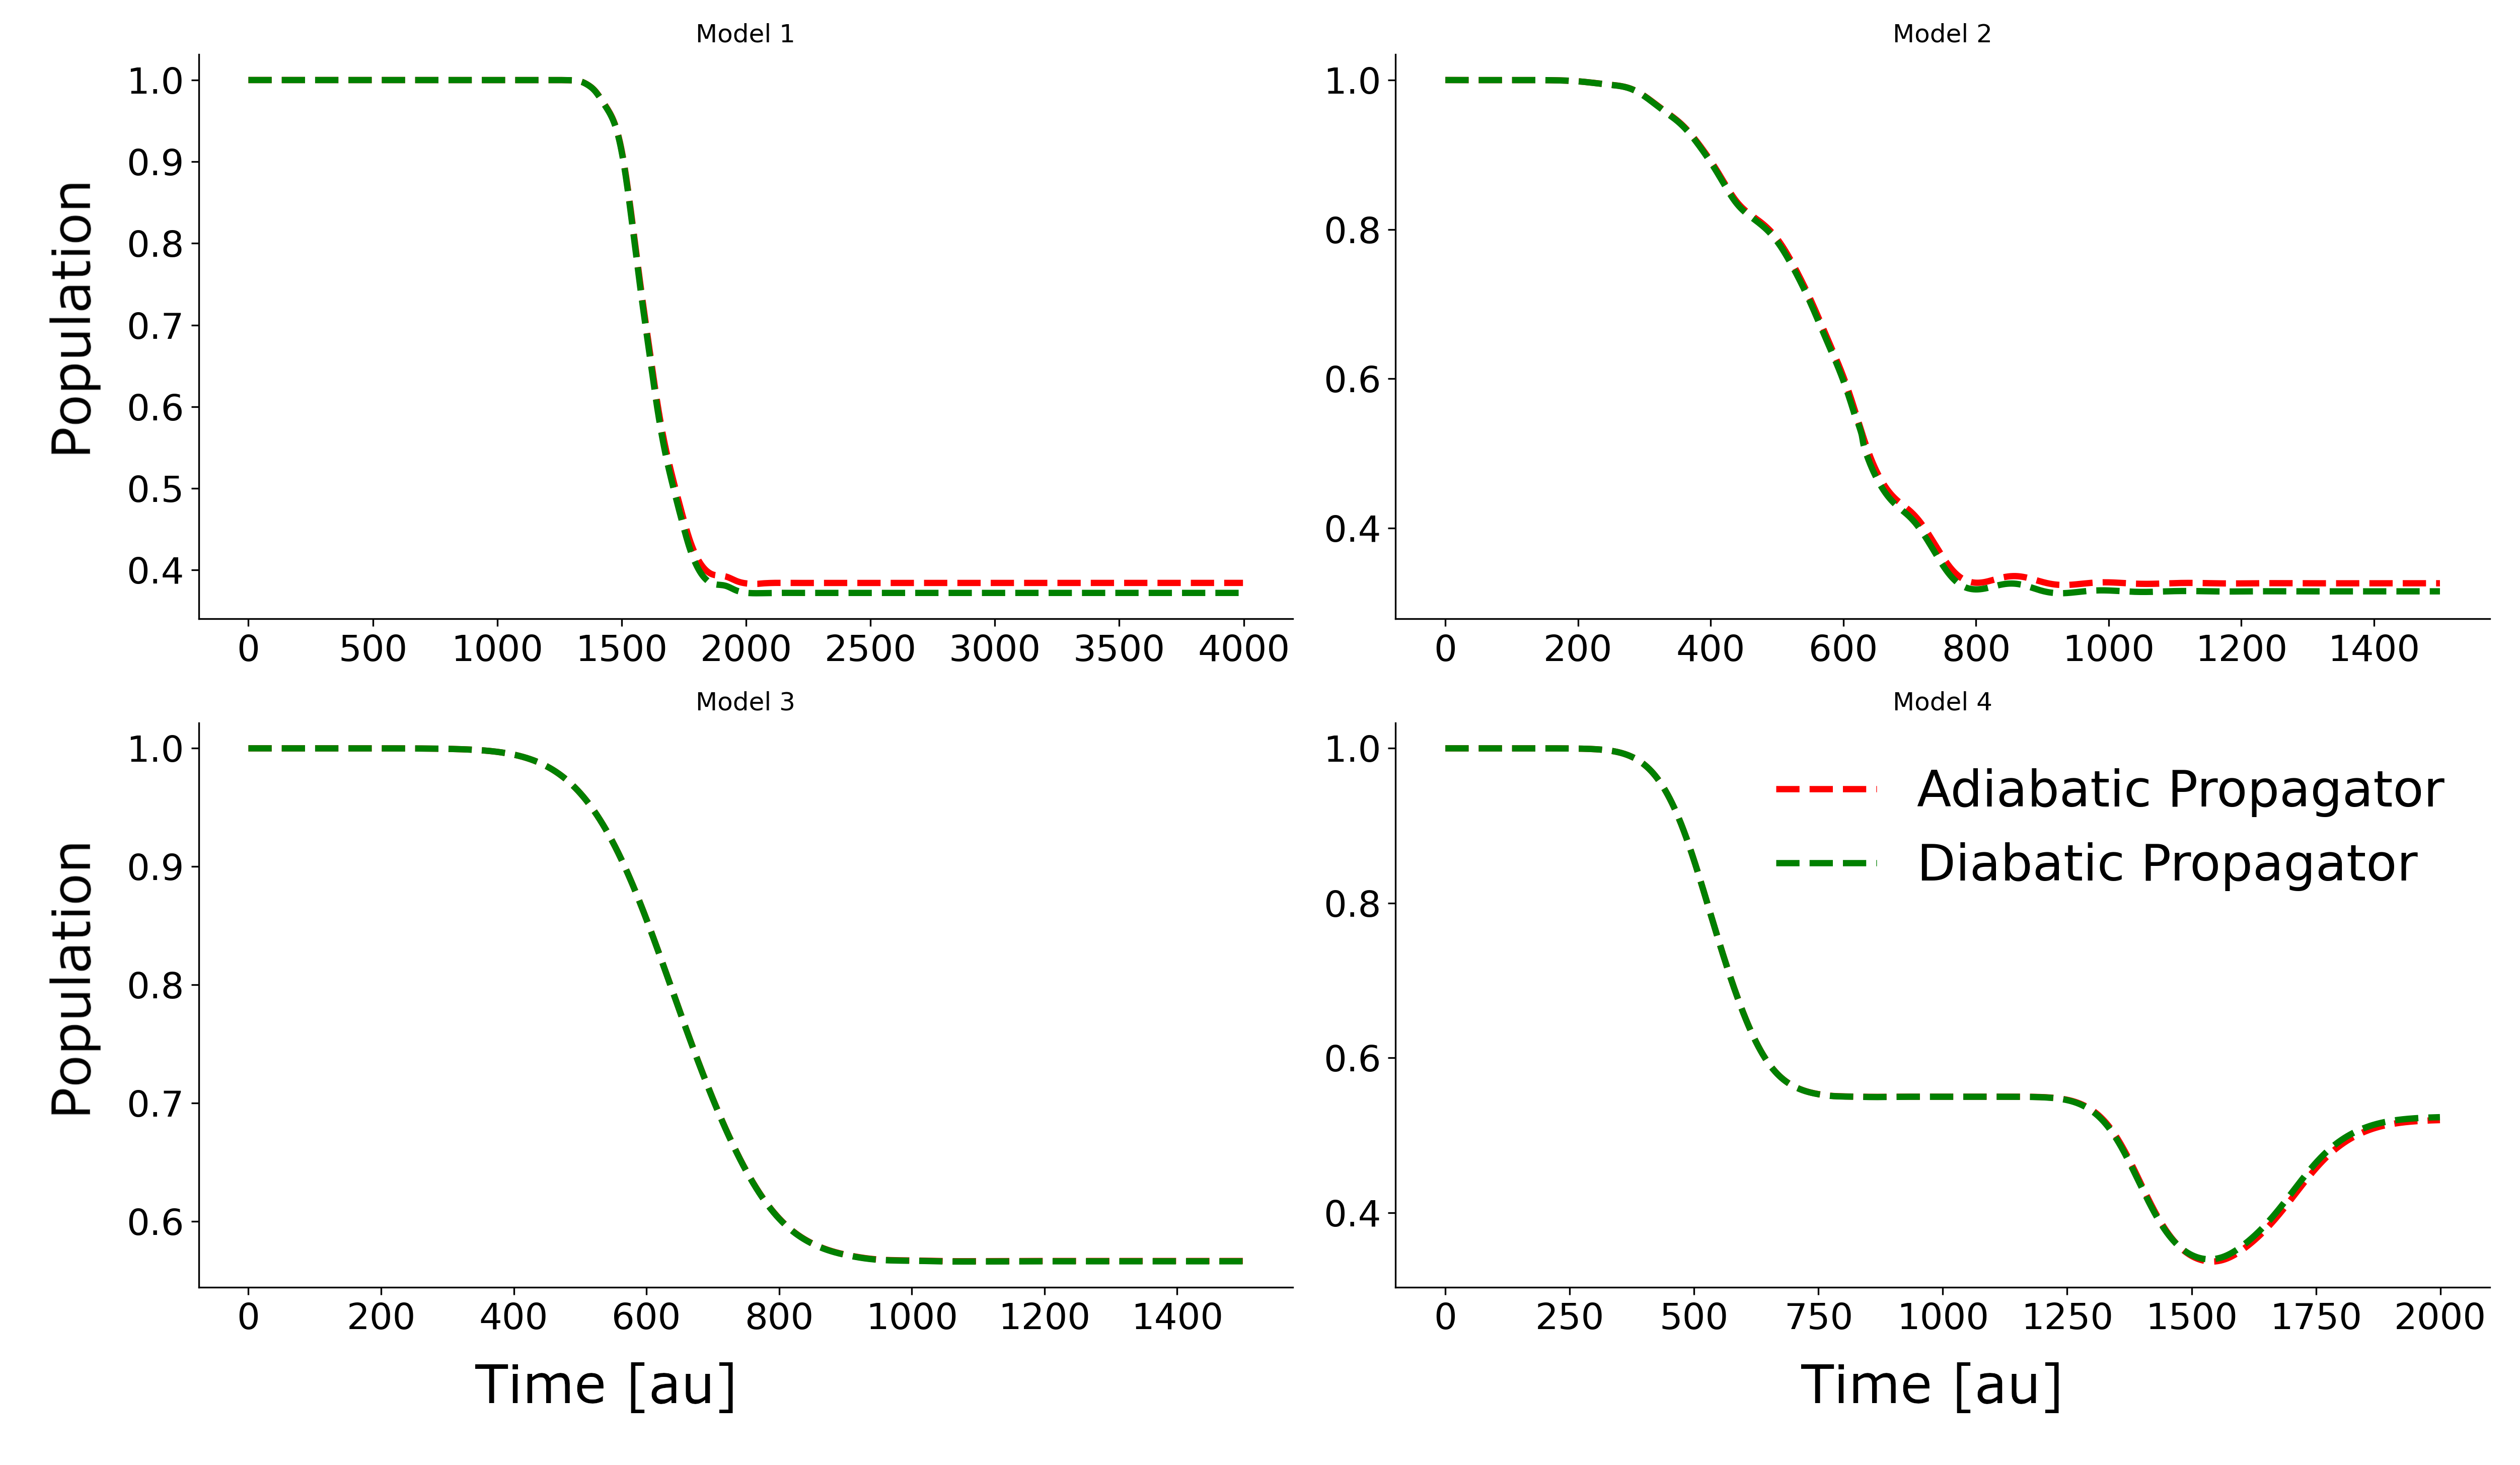
\includegraphics[width=\textwidth]{../img/CTMQC/TullyModels/CTMQC_ad_vs_di_wTraj_pops.png}
  \caption{\label{fig:diab_prop_vs_adiab}The 4 Tully models simulated using propagating the equations within a diabatic and adiabatic basis. The green line shows results from the diabatic propagator and the red line shows results from the adiabatic propagator. Model 3 shows an exact agreement between the adiabatic and diabatic propagators hence only 1 line is seen.}
\end{figure}
We can see in figure \ref{fig:diab_prop_vs_adiab} that the results for the adiabatic and diabatic propagator are almost exactly the same for each model. In model 3, where the problem with the divergent $\mathcal{Q}_{lk, \nu}^{(I)}$ doesn't occur, the 2 results are exactly on top of each other. In the other models there is a slight discrepancy. This is due to the unpredictable $\mathcal{Q}_{lk, \nu}^{(I)}$ spikes not being perfectly corrected. However, figure \ref{fig:diab_prop_vs_adiab} still serves as confirmation of the propagation within the diabatic basis.

\section{Simulating Molecular Systems}
To go beyond the 1D Tully model systems the AOM method is combined with CTMQC and applied to an Ethylene dimer. Fortunately, the majority of the code from the Tully model systems can be re-used. In fact, the only difference is the way the Hamiltonian (and diabatic NACE) is constructed. The code for carrying out these tasks (the AOM part) has been implemented by previous members of the group and has been well tested and verified against the literature and experimental studies. Therefore, I will not include any tests of this part of the code in this document but instead refer the reader to the numerous papers discussing AOM and its use in within the fewest switches surface hopping framework \cite{Carof2017FSSH, C9FD00046A, C9CP04770K, FOB-SH_Spencer, C6FD00107F,FlickPolarons, Giannini2018Crossover, Giannini2019, C9TC05270D,Gajdos2014, AOM_vs_HigherOrder}. An ethylene dimer was chosen as a reasonable first system due to its relative simplicity (shown in figure \ref{fig:EthDimer}) the total number of atoms is 12 and only 2 electronic states will be considered.
\begin{figure}[ht]
  \includegraphics[width=\textwidth]{../img/CTMQC/Ethylene_Annotated.png}
  \caption{\label{fig:EthDimer}An example Ethylene dimer used to test the CTMQC implementation. The right panel shows the positions of just 1 replica. The left panel shows the positions of all replica with the replica shown on the right highlighted in red.}
\end{figure}
The system shown in figure \ref{fig:EthDimer} was initialised in the adiabatic ground state. Positions and velocities were sampled from a short NVT molecular dynamics equilibration. The scaling factor ($C$ in equation \eqref{eq:AOM_proportional}) was chosen to give a coupling of approximately 27 meV. This is approximately $\frac{1}{4} \times$ the reorganisation energy -parameterised to be 100 meV. The amount of charge transfer is dependent on the ratio between reorganisation energy and the electronic couplings ($\frac{H_{ab}}{\lambda}$). The factor of $\frac{1}{4}$ was chosen to be a reasonable factor -seen in other organic semiconducting systems. The nuclear timestep was chosen to be 0.05fs and the electronic one was 0.005 fs. The switch to $\mathbf{R}_{0, \nu}^{(I)}$ was chosen as the correction method of the quantum momentum and 100 trajectories were used. A constant $\sigma$ of 0.7 was used as the dynamic $\sigma$ tended to either vanish to 0 or blow up to a very large number.
\\\\
In figure \ref{fig:CP2K_norm} the norm of the diabatic expansion coefficients are plotted, from the system described above. In this figure we see large jumps in the norm, these are caused by the divergences in the quantum momentum term. These occur more in this system than in the Tully models as it is more complex (more atoms, higher dimensional) and runs for a longer time with more avoided crossings. The fact that there are 12 atoms and 3 Cartesian dimensions instead of 1 means that the $\mathbf{R}_{lk, \nu}$ term must be calculated many more times increasing the probability of happening upon a divergence. For example, the Tully models tended to run for 10s of fs and had 1 value of $\mathbf{R}_{lk, \nu}$. The Ethylene dimer typically runs for 100s of fs encountering 10s of avoided crossings with 36 unique values of $\mathbf{R}_{lk, \nu}$. The errors can also accumulate meaning that after a few trivial crossings the populations become extremely noisy. This eventually causes the code to crash and results from it cannot be trusted. Most commonly the reason for the code crashing is a large spike in the computed forces caused by a spike in the quantum momentum. This large force then causes the atoms to collide and the code to crash. The code is very stable when just using Ehrenfest dynamics.
\begin{figure}[ht]
  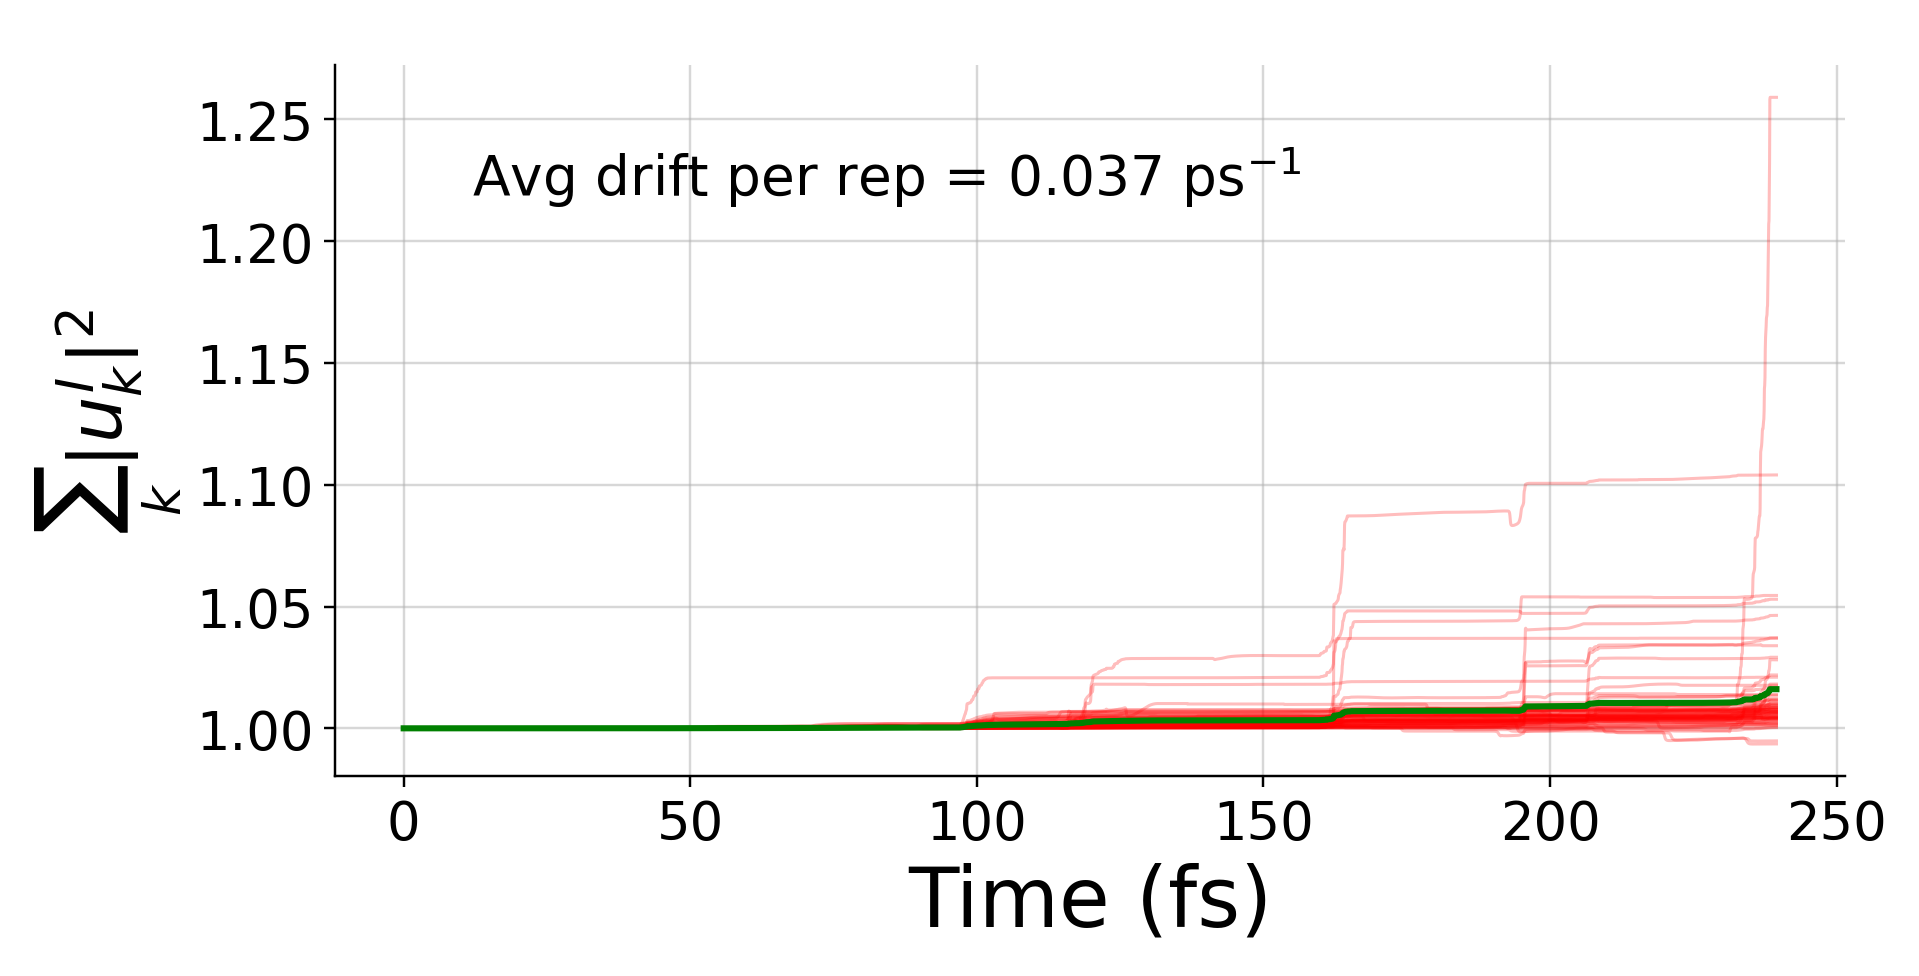
\includegraphics[width=\textwidth]{../img/CTMQC/Ethylene_norm.png}
  \caption{\label{fig:CP2K_norm}The norm of the adiabatic expansion coefficients. Thin red lines show the norm for each trajectory and the thick green line shows the average over all trajectories.}
\end{figure}
Many more simulations have been carried out to diagnose and fix this issue. Results from all of these cannot be included in this document though I will provide a brief summary of results below.
\\
\begin{itemize}
	\item \textbf{Varying the number of replicas}: Increasing the number of replicas in the system, somewhat counterintuitively, decreases stability. This is because with more replicas there is more of a chance the code will stumble upon a calculation giving a divergence in the quantum momentum term.
	\item \textbf{Varying the timestep}: Decreasing the timestep does help to improve norm conservation (before the code crashes). However, it does not lead to a more stable simulation that allows for longer timescales to be simulated. This is because decreasing the timestep provides more opportunity for a small numerical error to cause a divergence in the quantum momentum term.
	\item \textbf{Removing Center of Mass Motion}: In some simulations the replicas positions spread out so much that the quantum momentum term became negligible. This was to prevent that from happening.
	\item \textbf{Varying the gaussian width ($\sigma$) parameter}: If the $\sigma$ parameter is set to be large (> 2) then the simulation is more stable as the quantum momentum term is smaller and errors don't accumulate as quickly. However, this the limit of a very large $\sigma$ is Ehrenfest dynamics. If the $\sigma$ is set to be small (< 0.2) the simulation becomes extremely unstable as the quantum momentum forces populations to decohere too quickly. This is discussed in more detail in section \ref{sect:SigmaSect}.
	\item \textbf{Turning off the quantum momentum addition to the force term}: The code runs more stably if the quantum momentum term is not included in the forces. This has also been shown to be much less important for the accuracy of the results than the quantum momentum addition to the coefficients. However, even in this case the code eventually crashes after an accumulation of errors in the coefficients results in erroneous forces resulting in geometries that fail CP2K internal checks.
	\item \textbf{Renormalisation}: This does not seem to help with stability. Furthermore, it merely helps hide the large norm drift and doesn't fix the problems it causes.
\end{itemize}
\section{Conclusions}
The CTMQC method shows great promise as a new nonadiabatic molecular dynamics (NAMD) technique. It was derived as the semi-classical limit of the exact factorisation of the time-dependent electron-nuclear wave function \cite{abedi_exact_2010, agostini_semiclassical_2015}. It purports to handle decoherence corrections in a more rigorous, first principles, way without the need of empirical parameters. Although this method was first reported in 2015 \cite{agostini_semiclassical_2015}, there are still very few papers reporting results using this method \cite{min_ab_2017, gossel_coupled-trajectory_2018,agostini_semiclassical_2015}. With the most complex system being restricted to a 7 atom molecule simulated for just 10s of fs\cite{min_ab_2017}. In this work, I have transformed the basis of the CTMQC equations, to an orthogonal diabatic basis, and implemented it within the FOB framework. This has allowed me to study to a molecular system (dimer of Ethylene) totalling 12 atoms, simulated for hundreds of fs. However, instabilities in the algorithm have prevented any physical conclusions being drawn from this. Before the widespread acceptance of CTMQC as a standard nonadiabatic molecular dynamics method, 2 critical flaws must be addressed. First is the calculation of the gaussian width parameter, $\sigma$, and the second is the divergence of the quantum momentum term. It would be possible to further investigate the width parameter, perhaps through benchmarks against higher level calculations to establish a relationship between it and other characteristics of the system. From a short investigation using the Tully models it seems a constant width parameter gives reasonable results and it should be set to be between 0.2 and 0.5. The on-the-fly update of the width parameter, from an algorithm given in Gossel \cite{gossel_coupled-trajectory_2018}, provided even better results that came very close to the exact quantum dynamical values. Therefore, the setting of this width parameter does not seem like an intractable problem. However, it may be harder to correct for the large divergences in the quantum momentum caused by the denominator of the quantum momentum intercept term, $\mathbf{R}_{lk, \nu}$, approaching zero. This causes the code to become unstable for even simple molecular systems. In the 1D Tully models, this could be corrected by switching to an alternative intercept, $\mathbf{R}_{0, \nu}^{(I)}$. The switch occurs after 2 conditions are satisfied: a threshold on the time-derivative of the $\mathbf{R}_{lk, \nu}$ term has been surpassed and the denominator of the $\mathbf{R}_{lk, \nu}$ term is sufficiently close to 0. The correction helps conserve norm within the Tully model simulations. However, in larger, longer running simulations errors soon accumulate and the code becomes unstable. The Tully models also gave fewer divergences due to smaller run-times and the fact it is a simpler system. The alternative intercept results in unphysical population transfer in regions of zero nonadiabatic coupling, so cannot be used throughout the simulation.
\\\\
Both these problems can both be traced back to the construction of the nuclear density from the nuclear positions. The method explored in this thesis is the method reported in the literature. That involves placing a gaussian function centered on each atomic position with a certain width, $\sigma$ to smear out the (point) position and give a smooth nuclear distribution. I believe that exploring alternative techniques to construct the nuclear density from atomic positions may lead to the largest improvements in the CTMQC technique. Perhaps even allowing one to study complex molecular systems with many nonadiabatic coupling regions such as those typically found in charge transfer studies. 
\\\\
Finally, the algorithm does not seem to conserve total energy. Using the equation for potential energy given in \cite{agostini_semiclassical_2015} we see that even very small nuclear timesteps do not conserve total energy to better than 10$^{-2}$ Ha ps$^{-1}$ atom$^{-1}$ in the best case. For reference, a good energy conservation within classical molecular dynamics is considered to be $\sim 10^{-10}$ or less. Further, and perhaps more concerning, reducing the timestep does not seem to improve the issue. This would be a major obstacle to CTMQC's widespread adoption as a nonadiabatic molecular dynamics algorithm and further work is needed to address the issue. In the rest of this work I will discuss an alternative NAMD technique, namely fewest switches surface hopping (FSSH), and apply it to large molecular systems to get experimentally verifiable results.
\\\\
I have implemented and tested a working version of CTMQC both in CP2K and as a standalone python script. These are both available for downloading from the author's github page at: \href{https://github.com/95ellismle}{https://github.com/95ellismle}.
